% Beamer slide deck for Mathematical Physics
% "Mathematical Physics"
% Chapter 2: Gamma, Beta, Zeta
% Core Gamma + Beta, with a Zeta module.
% Mathematical text is self-contained; compilation also requires Kyushu.sty and the local PDFs under figs/.

\documentclass[11pt]{beamer}

\usepackage[utf8]{inputenc}
\usepackage[T1]{fontenc}
\usepackage{lmodern}
\usepackage{amsmath,amssymb}
\usepackage{graphicx}
\usepackage{tikz}
\usetikzlibrary{decorations.markings}

\usetheme{Madrid}

\author[]{Compiled by Jake W. Liu}
\title[Gamma, Beta, Zeta]{Chapter 2: Gamma, Beta, Zeta}
\subtitle{Mathematical Physics}
\date{\today}

\setbeamertemplate{navigation symbols}{}
\setbeamertemplate{frametitle continuation}[from second]

% Section mini-TOCs omitted to keep the deck compact; full outline is above.

\usepackage{Kyushu}

% Neutralize \index so source markup (if any) is harmless.
\makeatletter
\@ifundefined{index}{\newcommand{\index}[1]{}}{\renewcommand{\index}[1]{}}
\makeatother

\begin{document}

\newcounter{sfchapter}
\setcounter{sfchapter}{2}
\renewcommand{\thesection}{\arabic{sfchapter}.\arabic{section}}
\numberwithin{equation}{section}

\begin{frame}[c]\titlepage
\end{frame}

\begin{frame}{Outline}
\tableofcontents
\end{frame}

\begin{frame}{Where we are going}
\footnotesize
Many special functions begin as discrete objects---factorials, partial sums,
\(p\)-series---and gain power once they are extended to continuous (or complex)
arguments. This chapter develops the functions that form the basic
\emph{language} of that extension:
\begin{itemize}
  \item \textbf{Harmonic numbers} \(H_n=\sum_{k=1}^n\tfrac1k\) and the continuous
        interpolation that produces the Euler--Mascheroni constant \(\gamma\).
  \item The \textbf{gamma function} \(\Gamma(z)\): the canonical meromorphic
        interpolation of the shifted factorial. Integral definition, recursion,
        half-integers, poles, reflection, Euler's limit form, Hankel's contour for
        \(1/\Gamma\), and Stirling.
  \item The \textbf{beta function} \(B(p,q)\): the integral that encodes binomial
        structure, linked to gamma by \(B(p,q)=\Gamma(p)\Gamma(q)/\Gamma(p+q)\).
  \item \textbf{Riemann zeta function}
        \(\zeta(s)\) for \(\operatorname{Re}s>1\): series, integral representation,
        Euler product, and the Basel value \(\zeta(2)=\pi^2/6\).
\end{itemize}
The common question is how to extend a discrete pattern to a function we can
differentiate, integrate, and use in later chapters. Write \(\mathbb N=\{1,2,\dots\}\) and \(\mathbb N_0=\{0,1,2,\dots\}\).
\end{frame}


% ======================================================================
\section{Harmonic Numbers}
% ======================================================================

\begin{frame}[allowframebreaks=1.00]{Block stacking and the harmonic numbers}
\footnotesize

\textbf{Step 1: find the increment.}  How far can \(n\) identical blocks (length two units, unit mass) overhang a table edge?
With one block we balance it half off, so its center of mass sits at the edge \(x=0\); the
overhang is \(H_1=1\).

Suppose \(n-1\) stacked blocks already have their center of mass at the edge, with total
overhang \(H_{n-1}\). Slip one more block underneath with its center at \(-1\), so its right end
lines up with the table edge; the old stack still balances, now on that end. The new center of mass \(x\) of
all \(n\) blocks is the mass-weighted average (total mass \(n\) times \(x\) equals the sum of
mass times position): the top \(n-1\) blocks contribute mass \(n-1\) at position \(0\), and the
new block mass \(1\) at position \(-1\), so
\[
  n\,x = (n-1)\cdot 0 + 1\cdot(-1) \;\Longrightarrow\; x = -\tfrac1n .
\]
Shifting the whole stack forward by \(1/n\) returns its center of mass to the edge
and increases the overhang by the same amount. Thus
\(H_n=H_{n-1}+1/n\); starting from \(H_0=0\) and adding the increments,
\begin{equation}
  H_n = 1 + \tfrac12 + \tfrac13 + \tfrac14 + \cdots + \tfrac1n
      = \sum_{k=1}^{n}\frac1k .
  \label{eq:harmonic}
\end{equation}


\par\framebreak\par
\textbf{Step 2: name the sequence.}  The series \(1+\tfrac12+\tfrac13+\cdots\) is the \emph{harmonic series}; its partial sums
\eqref{eq:harmonic} are the \emph{harmonic numbers}
\(\{1,\tfrac32,\tfrac{11}{6},\tfrac{25}{12},\dots\}\). They diverge, but extraordinarily
slowly: we will see below that \(H_n\approx\log n+0.577\), so \(H_n>100\) (an overhang of
\(50\) block lengths) needs roughly \(1.5\times10^{43}\) blocks.

This raises two questions we now answer.
\begin{itemize}
  \item What natural analytic function interpolates the discrete sequence \(H_n\)?
  \item How slowly does the sequence diverge?
\end{itemize}
The harmonic series is the special case \(p=1\) of the \(p\)-series
\(\sum_{k=1}^{\infty}k^{-p}\), which reappears as the zeta function at the end of this chapter.
\end{frame}


\begin{frame}[allowframebreaks=1.00]{Interpolating the partial sums}
\footnotesize
\textbf{A finite sum as an integral.} The geometric identity gives
\[
 \frac{1-x^n}{1-x}=1+x+\cdots+x^{n-1}\qquad(x\neq1).
\]
At $x=1$ the left side is $0/0$, but the right side is a polynomial, so the gap
is a removable singularity: its continuous value there is $1+1+\cdots+1=n$. Integrating each power on $[0,1]$ gives
\[
 \int_0^1\frac{1-x^n}{1-x}\,dx
 =\sum_{k=0}^{n-1}\int_0^1x^k\,dx
 =\sum_{k=0}^{n-1}\frac1{k+1}=H_n .
\]
Nothing on the left needs $n$ to be an integer, which suggests the interpolation
\begin{equation}
 f(s)=\int_0^1\frac{1-x^s}{1-x}\,dx,\qquad \operatorname{Re}s>-1,
 \label{eq:harmonic-interp}
\end{equation}
where $x^s=e^{s\log x}$ uses the real logarithm on $0<x<1$, hence
$|x^s|=x^{\operatorname{Re}s}$. Only the endpoints can hurt. At zero the sole
possibly singular term is $x^s$, of size $x^{\operatorname{Re}s}$, and
$\int_0x^\sigma\,dx$ converges exactly for $\sigma>-1$ (at $\sigma=-1$ it is
$\int_0dx/x$). At one the gap is again removable: l'H\^opital's rule gives
$(1-x^s)/(1-x)\to s$.
Thus $f(n)=H_n$.
\par\framebreak\par
\textbf{The recursion survives.} The block-stacking recursion $H_n=H_{n-1}+1/n$ also extends to every $s$: subtract the integrand of \eqref{eq:harmonic-interp} at $s$ from the one at $s+1$,
\begin{align*}
 f(s+1)-f(s)&=\int_0^1\frac{(1-x^{s+1})-(1-x^s)}{1-x}\,dx
 =\int_0^1\frac{x^s(1-x)}{1-x}\,dx\\
 &=\int_0^1x^s\,dx=\frac1{s+1},\qquad f(0)=\int_0^1\frac{1-1}{1-x}\,dx=0.
\end{align*}
So $f$ answers the first question: it is a smooth ``$H_s$'' for noninteger $s$. For example,
with $x=u^2$ ($dx=2u\,du$) and $(1-u)/(1-u^2)=1/(1+u)$,
\[
 f\bigl(\tfrac12\bigr)=\int_0^1\frac{1-u}{1-u^2}\,2u\,du=2\int_0^1\Bigl(1-\frac1{1+u}\Bigr)du
 =2-2\log2\approx0.614,
\]
between $H_0=0$ and $H_1=1$. Once the gamma function is built below,
$f(s)=\Gamma'(s+1)/\Gamma(s+1)+\gamma$ (quoted; $\gamma\approx0.577$ is the constant found
next): $f$ is the bridge from $H_n$ to $\Gamma$.
\par\framebreak\par
\textbf{The difference between a staircase and a logarithm.}
Rewrite each term of $H_n$ as a width-one rectangle over $[k,k+1]$: the integrand
$1/k$ is constant in $x$, so $\int_k^{k+1}dx/k=1/k$---the same sum, dressed as an
area. On that interval the curve $1/x$ lies below the flat top
($1/x<1/k$ for $k<x<k+1$), so each rectangle overtops the curved sliver beneath
it and the areas compare term by term:
\[
 H_n=\sum_{k=1}^{n}\int_k^{k+1}\frac{dx}{k}
 >\sum_{k=1}^{n}\int_k^{k+1}\frac{dx}{x}
 =\int_1^{n+1}\frac{dx}{x}=\log(n+1)>\log n.
\]
The positive difference $a_n=H_n-\log n$ decreases, since
\[
 a_{n+1}-a_n=\frac1{n+1}-\bigl(\log(n+1)-\log n\bigr)
 =\int_n^{n+1}\Bigl(\frac1{n+1}-\frac1x\Bigr)dx<0,
\]
because $1/x>1/(n+1)$ for $n<x<n+1$.

A decreasing sequence bounded below (here by $0$, since $H_n>\log n$) has a limit. We call it the
Euler--Mascheroni constant:
\begin{equation}
 \gamma=\lim_{n\to\infty}(H_n-\log n)=0.577215664901532\ldots.
 \label{eq:euler-gamma}
\end{equation}

\end{frame}

\begin{frame}{Euler--Mascheroni as a staircase error}
\footnotesize
\begin{center}
  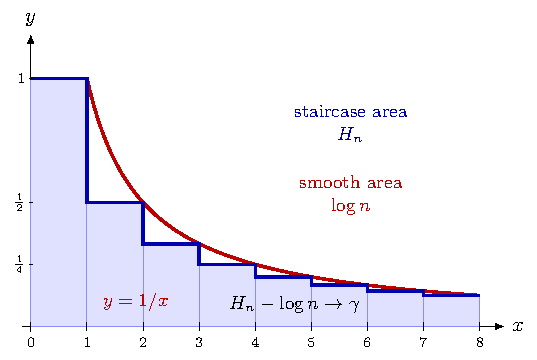
\includegraphics[width=0.68\linewidth]{figs/ch2_euler_gamma_staircase.pdf}
\end{center}
The harmonic number \(H_n\) is the area of a unit-width staircase. The logarithm
\(\log n=\int_1^n dx/x\) is the area under the smooth curve. The limiting excess area is
\(\gamma=\lim_{n\to\infty}\bigl(H_n-\log n\bigr)\).
\end{frame}


% ======================================================================
\section{Gamma Function}
% ======================================================================


\begin{frame}[allowframebreaks=1.00]{Definition and the factorial recursion}
\footnotesize

The factorial $n!$ gets the same treatment as $H_n$: write it as an integral in
which $n$ appears as an exponent, then let $n$ become a continuous variable.

\textbf{Step 1: define the interpolation.}  Which integral produces $n!$?
Integrating by parts lowers the power of $t$ by one at each step, so pair $t^n$
with a factor that reproduces itself under integration and dies at
$+\infty$---namely $e^{-t}$. Repeated application gives
\(\int_0^\infty t^ne^{-t}\,dt=n!\) (Steps~2--3 below: one integration by parts
yields the recursion, iterated to the base case), and the integral still makes
sense when \(n\) is not an integer. Replacing \(n\) by \(z-1\) (the historical convention) defines the
\emph{gamma function}, Euler's integral of the second kind,
\begin{equation}
  \Gamma(z)=\int_0^\infty e^{-t}t^{z-1}\,dt,
  \qquad \operatorname{Re}z>0.
  \label{eq:gamma-def}
\end{equation}
With \(\sigma=\operatorname{Re}z\): near \(t=0\) the integrand has size \(t^{\sigma-1}\), which is
integrable exactly when \(\sigma>0\); at infinity \(e^{-t}\) beats every power.
Infinitely many functions agree with \(n!\) at the integers; \(\Gamma\) is the standard one
because it is the only positive function on \(x>0\) with \(f(x+1)=xf(x)\), \(f(1)=1\) and
\(\log f\) convex (Bohr--Mollerup theorem, quoted).

\par\framebreak\par
\textbf{Step 2: derive the recursion.}  Integrate \(\Gamma(z+1)\) by parts with \(u=t^z\),
\(dv=e^{-t}dt\), so \(du=z\,t^{z-1}dt\) and \(v=-e^{-t}\):
\[
  \Gamma(z+1)
   =\int_0^\infty e^{-t}t^z\,dt
   =\left[-t^ze^{-t}\right]_{0}^{\infty}
     +z\int_0^\infty e^{-t}t^{z-1}\,dt.
\]
For \(\sigma>0\), \(|t^ze^{-t}|=t^\sigma e^{-t}\to0\) both as \(t\to0^+\) and as \(t\to\infty\),
so the boundary term is zero. Therefore
\begin{equation}
  \Gamma(z+1)=z\,\Gamma(z).
  \label{eq:gamma-rec}
\end{equation}

\textbf{Step 3: recover factorials.}  At \(z=1\),
\(\Gamma(1)=\int_0^\infty e^{-t}\,dt=\left[-e^{-t}\right]_{0}^{\infty}=1\).
For \(n\in\mathbb N\), repeated use of \eqref{eq:gamma-rec} gives
\[
  \Gamma(n+1)=n\,\Gamma(n)=n(n-1)\Gamma(n-1)=\cdots=n(n-1)\cdots2\cdot1\,\Gamma(1)=n!.
\]
Together with \(\Gamma(1)=1=0!\), this proves
\begin{equation}
  \Gamma(n+1)=n!,
  \qquad n=0,1,2,\dots .
  \label{eq:gamma-fact}
\end{equation}
Keep track of the shift: \(\Gamma(n+1)=n!\), not \(\Gamma(n)=n!\).
\end{frame}


\begin{frame}[allowframebreaks=1.00]{Worked examples: half-integer values}
\footnotesize

\textbf{Why half-integers.} The recursion turns every \(\Gamma(m+\tfrac12)\) into a
multiple of one base value, \(\Gamma(1/2)\) — the values that reappear in
\(J_{\pm1/2}\) (Chapter~3) and in the spherical-Bessel formulas of Chapter~5.
That base value turns out to be the Gaussian integral in disguise.

\textbf{Step 1: evaluate the Gaussian integral.}  Let
\(I=\int_{-\infty}^{\infty}e^{-x^2}\,dx\); the integrand is positive, so \(I>0\).
Squaring and writing the product as a double integral,
\begin{align*}
  I^2
   &=\left(\int_{-\infty}^{\infty}e^{-x^2}\,dx\right)
     \left(\int_{-\infty}^{\infty}e^{-y^2}\,dy\right)
    =\int_{\mathbb R^2}e^{-(x^2+y^2)}\,dx\,dy.
\end{align*}
In polar coordinates
\(x=r\cos\theta\), \(y=r\sin\theta\), a small area element has sides \(dr\) and
\(r\,d\theta\), hence \(dx\,dy=r\,dr\,d\theta\). Thus
\[
  I^2
   =\int_0^{2\pi}\int_0^\infty e^{-r^2}r\,dr\,d\theta
   =\int_0^{2\pi}
     \left[-\frac12e^{-r^2}\right]_{r=0}^{r=\infty}d\theta
   =\int_0^{2\pi}\frac12\,d\theta
    =\pi,
\]
and because \(I>0\),
\begin{equation}
  \int_{-\infty}^{\infty}e^{-x^2}\,dx=\sqrt\pi .
  \label{eq:gauss-int}
\end{equation}

\textbf{Step 2: a Gaussian form of \(\Gamma\), at \(z=\tfrac12\).}  Put \(t=u^2\) in \eqref{eq:gamma-def},
so \(dt=2u\,du\) and \(t^{z-1}=u^{2z-2}\) for \(u>0\):
\begin{equation}
  \Gamma(z)=\int_0^\infty e^{-u^2}u^{2z-2}(2u)\,du
  =2\int_0^\infty e^{-u^2}u^{2z-1}\,du,
  \qquad \operatorname{Re}z>0.
  \label{eq:gamma-gauss}
\end{equation}
At \(z=\tfrac12\), \(2z-1=0\); since \(e^{-u^2}\) is even, \eqref{eq:gauss-int} gives
\begin{equation}
  \Gamma\left(\tfrac12\right)=2\int_0^\infty e^{-u^2}\,du
  =\int_{-\infty}^{\infty}e^{-u^2}\,du=\sqrt\pi.
  \label{eq:gamma-half}
\end{equation}
One application of the recursion \eqref{eq:gamma-rec}, written as
\(\Gamma(z)=(z-1)\,\Gamma(z-1)\) at \(z=\tfrac32\), gives
\(\Gamma(\tfrac32)=\tfrac12\,\Gamma(\tfrac12)=\sqrt\pi/2\).
Applying it \(m\) times in the same way,
\[
 \Gamma\left(m+\tfrac12\right)
 =\left(m-\tfrac12\right)\left(m-\tfrac32\right)\cdots\tfrac12\;
  \Gamma\left(\tfrac12\right)
 =\frac{1\cdot3\cdots(2m-1)}{2^m}\sqrt\pi,
\]
since each of the \(m\) factors is (odd number)\(/2\).
To put it in closed form, separate the even and odd factors of $(2m)!$; the even ones give
$2\cdot4\cdots(2m)=2^m m!$, so
\[
 (2m)!=(2^m m!)\,[1\cdot3\cdots(2m-1)]
 \quad\Longrightarrow\quad
 \frac{1\cdot3\cdots(2m-1)}{2^m}=\frac{(2m)!}{2^m m!\,2^m},
\]
and therefore
\[
 \Gamma\left(m+\tfrac12\right)=\frac{(2m)!}{4^m m!}\sqrt\pi .
\]
For example, $m=2$ gives $\Gamma(\tfrac52)=\tfrac{24}{16\cdot2}\sqrt\pi=\tfrac34\sqrt\pi$, which is
$\tfrac32\cdot\tfrac12\sqrt\pi$ as the recursion says. The formula also holds at $m=0$.
\end{frame}


\begin{frame}[allowframebreaks=1.00]{Analytic continuation to the left half-plane}
\footnotesize

\textbf{Why continue.} Bessel series (Chapters~3 and~5) contain \(\Gamma\) at negative
noninteger arguments, where the integral \eqref{eq:gamma-def} diverges. The outcome, plotted
after, is a function with poles at \(0,-1,-2,\dots\) whose sign alternates between them.

\textbf{Run the recursion backward.} Dividing \eqref{eq:gamma-rec} by \(z\),
\(\Gamma(z)=\Gamma(z+1)/z\), and \(\Gamma(z+1)\) is given by the integral whenever
\(\operatorname{Re}(z+1)>0\):
\[
  \Gamma(z)=\frac{\Gamma(z+1)}{z}
           =\frac1z\int_0^\infty e^{-t}t^z\,dt,
  \qquad \operatorname{Re}z>-1,\quad z\neq0.
\]
Repeating the recursion \(m\) times gives
\begin{align*}
  \Gamma(z+m)
   &=(z+m-1)\Gamma(z+m-1)
   =(z+m-1)(z+m-2)\Gamma(z+m-2)\\
   &=\cdots
    =(z+m-1)(z+m-2)\cdots(z+1)z\,\Gamma(z).
\end{align*}
If \(m\) is chosen so that \(\operatorname{Re}(z+m)>0\), then
\(\Gamma(z+m)\) is defined by the original integral and
\begin{equation}
  \Gamma(z)
   =\frac{\Gamma(z+m)}
          {z(z+1)(z+2)\cdots(z+m-1)}.
  \label{eq:gamma-continue}
\end{equation}
This defines \(\Gamma\) on the whole plane except \(0,-1,-2,\dots\) (a larger \(m\) gives the
same value, by the recursion).

\textbf{Poles and residues.} Near \(z=-n\), \(n\in\mathbb N_0\), set \(z=-n+\varepsilon\) and choose
\(m=n+1\) in \eqref{eq:gamma-continue}:
\[
  \Gamma(-n+\varepsilon)
   =\frac{\Gamma(1+\varepsilon)}
     {(-n+\varepsilon)(1-n+\varepsilon)\cdots(-1+\varepsilon)\,\varepsilon}.
\]
As \(\varepsilon\to0\), the numerator tends to \(\Gamma(1)=1\), and the \(n\) factors before
\(\varepsilon\) tend to \((-n)(1-n)\cdots(-1)=(-1)^n n!\) (an empty product \(1\) when \(n=0\)).
Hence the blow-up is a constant times \(1/\varepsilon\) — first power of the distance to \(-n\),
i.e.\ a \emph{simple pole}: using \(1/(-1)^n=(-1)^n\),
\[
  \Gamma(-n+\varepsilon)\approx\frac{(-1)^n}{n!\,\varepsilon}\qquad(\varepsilon\to0).
\]
Multiplying by \(\varepsilon=z-(-n)\) annihilates the finite part (\(\varepsilon\cdot\text{finite}\to0\))
and isolates the coefficient of \(1/\varepsilon\), the \emph{residue} — the only coefficient a
contour integral sees, since on a small circle every \(\varepsilon^k\) integrates to zero except
\(\varepsilon^{-1}\to2\pi i\):
\begin{equation}
  \operatorname*{Res}_{z=-n}\Gamma(z)=\lim_{\varepsilon\to0}\varepsilon\,\Gamma(-n+\varepsilon)=\frac{(-1)^n}{n!}.
  \label{eq:gamma-residue}
\end{equation}
\end{frame}

\begin{frame}{Real-axis picture of $\Gamma$}
\footnotesize
\begin{center}
  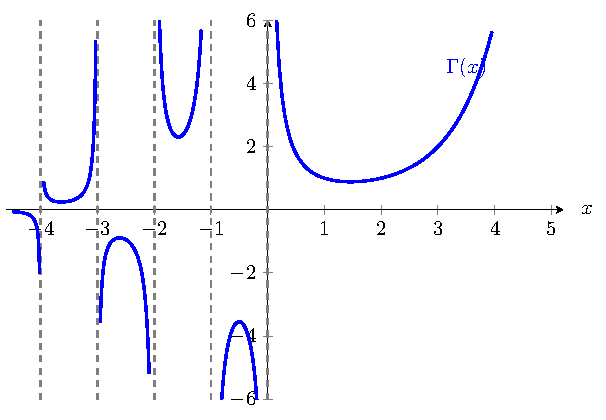
\includegraphics[width=0.62\linewidth]{figs/gamma-real.pdf}
\end{center}
On the positive real axis, \(\Gamma(n+1)=n!\). For \(-n<x<-n+1\), write
\(\Gamma(x)=\Gamma(x+n+1)/\bigl(x(x+1)\cdots(x+n)\bigr)\) by \eqref{eq:gamma-continue}: the numerator is
positive (\(x+n+1\) lies in \((1,2)\)), and exactly \(n\) of the factors, \(x,\dots,x+n-1\), are negative.
So \(\Gamma\) has sign \((-1)^n\) there, and runs off to \(\pm\infty\) at each end (the poles \eqref{eq:gamma-residue}).
\end{frame}


\begin{frame}[allowframebreaks=1.00]{Euler's reflection formula}
\footnotesize
\textbf{Why we want it.} The continuation reaches the left half-plane only by repeated division.
The reflection formula links \(\Gamma(z)\) directly to \(\Gamma(1-z)\), where \(1-z\) is the point
symmetric to \(z\) about \(\tfrac12\). Chapters~3 and~5 use it for the Airy and Bessel Wronskians.
\begin{block}{Euler's reflection formula}
\vspace{-1.2ex}
\begin{equation}
  \Gamma(z)\Gamma(1-z)=\frac{\pi}{\sin(\pi z)},\qquad z\notin\mathbb Z.
  \label{eq:gamma-reflect}
\end{equation}
\end{block}
Check at \(z=\tfrac12\): \(\Gamma(\tfrac12)^2=\pi/\sin(\pi/2)=\pi\), in agreement with \eqref{eq:gamma-half}.

\textbf{Proof for real \(0<a<1\).} With \(\Gamma(1-a)=\int_0^\infty s^{-a}e^{-s}\,ds\)
(\eqref{eq:gamma-def} at \(z=1-a\)), the product is
\[
  \Gamma(a)\Gamma(1-a)
   =\int_0^\infty\!\!\int_0^\infty
      t^{a-1}s^{-a}e^{-(t+s)}\,dt\,ds.
\]
To collapse the double integral, set \(t=su\) for each fixed \(s>0\), so \(s\)
survives only in the exponential. Then \(dt=s\,du\), \(e^{-(t+s)}=e^{-s(1+u)}\), and
\(t^{a-1}s^{-a}\,dt=(su)^{a-1}s^{-a}(s\,du)=u^{a-1}\,du\). Doing the \(s\)-integral first
(positive integrand, so the order may be swapped),
with \(\int_0^\infty e^{-s(1+u)}\,ds=1/(1+u)\),
\[
  \Gamma(a)\Gamma(1-a)
   =\int_0^\infty u^{a-1}
      \left(\int_0^\infty e^{-s(1+u)}\,ds\right)du
   =\int_0^\infty\frac{u^{a-1}}{1+u}\,du.
\]
Chapter~1 evaluated, by a keyhole contour,
\(\int_0^\infty x^{-b}(1+x)^{-1}dx=\pi/\sin(\pi b)\) for \(0<b<1\).
Taking \(b=1-a\), so that \(x^{-b}=x^{a-1}\) and \(\sin(\pi-\pi a)=\sin(\pi a)\), gives
\(\Gamma(a)\Gamma(1-a)=\pi/\sin(\pi a)\).

\textbf{All \(z\notin\mathbb Z\).} Both sides are analytic on the connected open set
\(\mathbb C\setminus\mathbb Z\) and agree on the segment \((0,1)\). By the identity theorem
(Chapter~1: two functions that agree on a segment agree on their whole connected
domain), they agree at every noninteger \(z\).

\textbf{Consequence: \(\Gamma\) has no zeros.} At a noninteger \(z\) the product
\(\Gamma(z)\Gamma(1-z)=\pi/\sin(\pi z)\) is nonzero, so neither factor vanishes. At positive integers
\(\Gamma(n)=(n-1)!\neq0\) by \eqref{eq:gamma-fact}; the remaining integers are poles.

\textbf{The form for \(\Gamma(-z)\).} Replacing \(z\) by \(-z\) in \eqref{eq:gamma-reflect} gives
$\Gamma(-z)\Gamma(1+z)=\pi/\sin(-\pi z)=-\pi/\sin(\pi z)$ (sine is odd); dividing by
$\Gamma(z+1)\neq0$,
\begin{equation}
 \Gamma(-z)=-\frac{\pi}{\Gamma(z+1)\sin(\pi z)},\qquad z\notin\mathbb Z.
 \label{eq:gamma-neg}
\end{equation}
It computes \(\Gamma\) at negative arguments from positive ones: at \(z=\tfrac12\),
\(\Gamma(-\tfrac12)=-\pi/\Gamma(\tfrac32)=-2\sqrt\pi\approx-3.54\), negative as the picture shows on \((-1,0)\).
\end{frame}


\begin{frame}[allowframebreaks=1.00]{Euler's limit representation}
\footnotesize
\textbf{What it is for.} It writes \(\Gamma\) as a limit of finite products, so the poles at
\(0,-1,-2,\dots\) show up openly as zeros of the denominator, and one formula covers every
\(z\) where \(\Gamma\) is finite, with no integral to converge.

\textbf{Goal.} Show that
\[
 \Gamma(z)=\lim_{n\to\infty}\frac{n^z\,n!}{z(z+1)\cdots(z+n)},
 \qquad z\notin\{0,-1,-2,\dots\}.
\]
The plan: replace \(e^{-t}\) in Euler's integral \eqref{eq:gamma-def} by a finite-\(n\) look-alike whose
integral can be done exactly, because it is a polynomial times a power of \(t\) (Steps~1--2); then
remove the restriction \(\operatorname{Re}z>0\) (Step~3).

\textbf{Step 1: truncate the exponential.} Since \((1-t/n)^n\to e^{-t}\), define, for
\(\operatorname{Re}z>0\),
\[
 F_n(z)=\int_0^n\left(1-\frac{t}{n}\right)^n t^{z-1}\,dt
 \;\longrightarrow\;\int_0^\infty e^{-t}t^{z-1}\,dt=\Gamma(z)\qquad(n\to\infty).
\]
(Since \((1-t/n)^n\le e^{-t}\), the limit can go inside the integral.)

\textbf{Step 2: evaluate \(F_n\) exactly.} Put \(t=nu\), so \(dt=n\,du\) and
\((nu)^{z-1}=n^{z-1}u^{z-1}\):
\(F_n(z)=n^z\int_0^1(1-u)^n u^{z-1}\,du\).
Integrate by parts with \(u^{z-1}\,du=d(u^z)/z\); the endpoint term vanishes, since
\((1-u)^n=0\) at \(u=1\) and \(u^z\to0\) at \(u=0\):
\[
 \int_0^1(1-u)^n u^{z-1}\,du
 =\left[\frac{(1-u)^n u^z}{z}\right]_0^1
  +\frac{n}{z}\int_0^1(1-u)^{n-1}u^z\,du
 =\frac{n}{z}\int_0^1(1-u)^{n-1}u^z\,du .
\]
Each such step lowers the power of \(1-u\) by one and raises that of \(u\) by one.
After \(n\) steps the factors \(\frac{n}{z}\cdot\frac{n-1}{z+1}\cdots\frac{1}{z+n-1}\) remain in front of
\(\int_0^1u^{z+n-1}\,du=\frac1{z+n}\), so
\[
 \int_0^1(1-u)^n u^{z-1}\,du=\frac{n!}{z(z+1)\cdots(z+n)},
 \qquad
 F_n(z)=\frac{n^z n!}{z(z+1)\cdots(z+n)}.
\]
Since \(F_n(z)\to\Gamma(z)\) for \(\operatorname{Re}z>0\) (Step~3 removes this restriction),
\begin{equation}
 \Gamma(z)=\lim_{n\to\infty}\frac{n^z n!}{z(z+1)\cdots(z+n)},
 \qquad z\notin\{0,-1,-2,\ldots\}.
 \label{eq:gamma-euler-limit}
\end{equation}
\textbf{Step 3: every \(z\) off the poles.} For \(\operatorname{Re}z\le0\) with
\(z\notin\{0,-1,-2,\dots\}\), pick \(m\) with \(\operatorname{Re}(z+m)>0\). Step~2's limit then
applies to \(\Gamma(z+m)\), and the continuation rule \eqref{eq:gamma-continue} divides it
by \(z(z+1)\cdots(z+m-1)\):
\[
 \Gamma(z)=\frac{\Gamma(z+m)}{z(z+1)\cdots(z+m-1)}
 =\lim_{n\to\infty}\frac{n^{z+m}n!}{z(z+1)\cdots(z+n+m)} ;
\]
the denominator concatenates the \(m\) new factors with the \(n+1\) factors
\((z+m)\cdots(z+m+n)\) of the \(\Gamma(z+m)\) approximant, so it runs from \(z\) to
\(z+m+n\). Peeling off its last \(m\) factors shows this approximant is just Step~2's
\(F_n(z)\) times \(m\) correction factors:
\[
 \frac{n^{z+m}n!}{z(z+1)\cdots(z+n+m)}
 =\underbrace{\frac{n^{z}n!}{z(z+1)\cdots(z+n)}}_{=\,F_n(z)}
 \;\prod_{j=1}^{m}\frac{n}{z+n+j},
 \qquad \frac{n}{z+n+j}\longrightarrow1 .
\]
Only \(m\) factors, each tending to \(1\), so the product tends to \(1\): the limit is
again \eqref{eq:gamma-euler-limit}, now for every \(z\) where \(\Gamma\) is finite.
\end{frame}


\begin{frame}[allowframebreaks=1.00]{Hankel's contour formula for $1/\Gamma$}
\footnotesize
\textbf{Why we want it.} Euler's integral \eqref{eq:gamma-def} needs \(\operatorname{Re}z>0\).
Hankel's integral gives \(1/\Gamma(a)\) for \emph{every} complex \(a\) in one formula, and in
Chapter~5 it turns a Bessel integral of noninteger order into its power series, one \(1/\Gamma\)
factor per term. The idea is Chapter~1's keyhole contour, opened up.

\textbf{What we will prove.} For every complex number \(a\),
\[
  \frac1{\Gamma(a)}=\frac1{2\pi i}\int_{\mathcal H}e^{t}\,t^{-a}\,dt,
\]
where \(\mathcal H\) is the loop contour of Step~1 (the numbered form is
\eqref{eq:hankel-gamma} at the end of Step~2).

\textbf{Where \(e^tt^{-a}\) comes from.} Euler's integral \eqref{eq:gamma-def} at \(z=1-a\) reads
\(\Gamma(1-a)=\int_0^\infty e^{-r}r^{-a}\,dr\). The substitution \(t=-r\) moves it to the negative
real axis, where \(e^{-r}=e^{t}\) and \(r^{-a}=(-t)^{-a}\): so \(e^tt^{-a}\) is Euler's integrand
in disguise. That integral converges only for \(\operatorname{Re}a<1\), because \(r^{-a}\)
blows up at \(r=0\). Hankel's idea is to go \emph{around} the troublesome point \(t=0\) instead
of running into it. Since \(t^{-a}\) takes different values on the two sides of the negative axis
(phases \(e^{\pm i\pi a}\), computed in Step~2), the two legs of the loop do not cancel; they
leave a factor \(\sin(\pi a)\), which the reflection formula \eqref{eq:gamma-reflect}
turns into \(1/\Gamma(a)\).

\par\framebreak\par
\begin{columns}[T]
\begin{column}{0.60\textwidth}
\textbf{Step 1: the contour.} The integrand has a branch point at \(t=0\), because
\(t^{-a}=e^{-a\log t}\) is multivalued unless \(a\) is an integer. Cut the plane along the
negative real axis and fix the branch with \(-\pi<\arg t<\pi\). The Hankel contour \(\mathcal H\)
comes in from \(-\infty\) \emph{below} the cut, circles the origin counterclockwise, and returns
to \(-\infty\) \emph{above} the cut. The loop stays away from \(t=0\), and on both legs \(e^t\)
decays like \(e^{-|t|}\) while \(t^{-a}\) grows at most like a power of \(|t|\), so the integral of
\(e^tt^{-a}\) converges for every complex \(a\); differentiating under the integral sign shows
that it is an entire function of \(a\).
\end{column}
\begin{column}{0.38\textwidth}
\centering
\begin{tikzpicture}[scale=0.62,>=stealth]
  \draw[->,gray] (-3.3,0)--(1.3,0) node[right]{\scriptsize$\operatorname{Re}t$};
  \draw[->,gray] (0,-1.3)--(0,1.3) node[above]{\scriptsize$\operatorname{Im}t$};
  \draw[orange!80!black,very thick] (-3.3,0)--(0,0);
  \node[orange!80!black,font=\scriptsize] at (-2.4,-0.95) {cut};
  \draw[blue!70!black,thick,decoration={markings,
      mark=at position 0.22 with {\arrow{>}},
      mark=at position 0.52 with {\arrow{>}},
      mark=at position 0.84 with {\arrow{>}}},postaction={decorate}]
    (-3.3,-0.3)--(-0.52,-0.3) arc[start angle=-150,end angle=150,radius=0.6]--(-3.3,0.3);
  \node[blue!70!black,font=\scriptsize] at (0.95,0.75) {$\mathcal H$};
  \fill (0,0) circle (1.5pt);
\end{tikzpicture}
\end{column}
\end{columns}

\smallskip
\textbf{Step 2: collapse onto the cut for \(0<a<1\).} For \(0<a<1\) the two legs become Euler
integrals we already know, so we compute there first and extend in Step~3. The aim of this step is
\(\int_{\mathcal H}e^tt^{-a}\,dt=2i\sin(\pi a)\,\Gamma(1-a)\). The integrand is holomorphic off the cut,
so by Cauchy's theorem (Chapter~1) the radius \(\varepsilon\) of the circle does not matter; shrink it.
On the lower leg \(t=re^{-i\pi}\) with \(r:\infty\to\varepsilon\); on the upper leg \(t=re^{i\pi}\) with
\(r:\varepsilon\to\infty\). On both, \(t=-r\), so \(e^t=e^{-r}\) and \(dt=-dr\), while
\(t^{-a}=r^{-a}e^{\pm i\pi a}\):
\begin{align*}
 \int_{\mathrm{lower}}e^t t^{-a}\,dt
 &=\int_\infty^\varepsilon e^{-r}\,r^{-a}e^{i\pi a}\,(-dr)
 =e^{i\pi a}\int_\varepsilon^\infty e^{-r}r^{-a}\,dr,\\
 \int_{\mathrm{upper}}e^t t^{-a}\,dt
 &=\int_\varepsilon^\infty e^{-r}\,r^{-a}e^{-i\pi a}\,(-dr)
 =-e^{-i\pi a}\int_\varepsilon^\infty e^{-r}r^{-a}\,dr.
\end{align*}
The circle contributes at most \(2\pi\varepsilon\cdot e^{\varepsilon}\varepsilon^{-a}\to0\), since \(a<1\).
Adding the legs and letting \(\varepsilon\to0\), with \(e^{i\theta}-e^{-i\theta}=2i\sin\theta\) and
\eqref{eq:gamma-def} at \(z=1-a\), gives \(\int_{\mathcal H}e^tt^{-a}\,dt=2i\sin(\pi a)\,\Gamma(1-a)\).
Divide by \(2\pi i\); by \eqref{eq:gamma-reflect} in the form \(\sin(\pi a)\Gamma(1-a)=\pi/\Gamma(a)\),
the result \(\sin(\pi a)\Gamma(1-a)/\pi\) equals \(1/\Gamma(a)\):
\begin{equation}
 \frac1{2\pi i}\int_{\mathcal H}e^t t^{-a}\,dt=\frac1{\Gamma(a)}.
 \label{eq:hankel-gamma}
\end{equation}

\textbf{Step 3: extend to every \(a\).} Step~2 proved the formula only for \(0<a<1\). The left side
is entire in \(a\) (Step~1); so is the right side, because \(\Gamma\) has no zeros, so \(1/\Gamma\)
has no poles (at the poles of \(\Gamma\) it is \(0\)). The two sides agree on \((0,1)\), so the identity theorem extends
\eqref{eq:hankel-gamma} to all complex \(a\).
\end{frame}


\begin{frame}[allowframebreaks=1.00]{Worked examples: gamma integrals}
\footnotesize

\textbf{Example 1.} Evaluate \(\int_0^\infty e^{-x^p}\,dx\) for \(p>0\).
Set \(t=x^p\), so \(x=t^{1/p}\), \(dx=\frac1p t^{1/p-1}\,dt\), and \(0,\infty\) map to \(0,\infty\). By \eqref{eq:gamma-def} with \(z=1/p\), and
then the recursion \eqref{eq:gamma-rec} in the form \(\frac1p\Gamma(\frac1p)=\Gamma(1+\frac1p)\),
\begin{equation}
  \int_0^\infty e^{-x^p}\,dx
   =\frac1p\int_0^\infty e^{-t}t^{1/p-1}\,dt
   =\frac1p\,\Gamma\left(\frac1p\right)
   =\Gamma\left(1+\frac1p\right).
  \label{eq:exp-xp}
\end{equation}
At \(p=2\) this is \(\Gamma(\tfrac32)=\sqrt\pi/2\), half of the Gaussian integral \eqref{eq:gauss-int}.

\begin{columns}[T]
\begin{column}{0.68\textwidth}
\textbf{Example 2: oscillation turned into decay.} For \(p>1\), evaluate \(\int_0^\infty\cos(x^p)\,dx\),
the real part of \(\int_0^\infty e^{ix^p}dx\). The integrand only oscillates, but on the ray at angle
\(\pi/(2p)\) it decays like \(e^{-r^p}\), which Example~1 handles. So close the sector in the
figure (principal branch \(z^p=e^{p\operatorname{Log}z}\); the small arc avoids the branch
point \(0\)).
\end{column}
\begin{column}{0.30\textwidth}
\centering
\begin{tikzpicture}[scale=0.75,>=stealth]
  \draw[->,gray] (-0.2,0)--(3.2,0) node[above]{\scriptsize$\operatorname{Re}z$};
  \draw[->,gray] (0,-0.2)--(0,1.9);
  \draw[blue!70!black,thick,decoration={markings,
      mark=at position 0.2 with {\arrow{>}},
      mark=at position 0.47 with {\arrow{>}},
      mark=at position 0.75 with {\arrow{>}}},postaction={decorate}]
    (0.35,0)--(2.7,0) arc[start angle=0,end angle=35,radius=2.7]--(35:0.35)
    arc[start angle=35,end angle=0,radius=0.35];
  \draw[gray] (0.9,0) arc[start angle=0,end angle=35,radius=0.9];
  \node[font=\scriptsize] at (1.45,0.35) {$\tfrac{\pi}{2p}$};
  \node[font=\scriptsize] at (2.7,-0.25) {$R$};
  \node[font=\scriptsize] at (0.35,-0.25) {$\varepsilon$};
\end{tikzpicture}
\end{column}
\end{columns}

On the slanted ray \(z=re^{i\pi/(2p)}\) we have \(z^p=r^p e^{i\pi/2}=ir^p\), so \(iz^p=-r^p\), and
\(dz=e^{i\pi/(2p)}\,dr\). By \eqref{eq:exp-xp}, the outward ray integral is
\[
  \int_{\mathrm{ray}}e^{iz^p}\,dz
   =e^{i\pi/(2p)}\int_0^\infty e^{-r^p}\,dr
   =e^{i\pi/(2p)}\,\Gamma\left(1+\frac1p\right).
\]
\par\framebreak\par
On the outer arc \(z=Re^{i\theta}\), \(0\le\theta\le\pi/(2p)\):
\(\operatorname{Re}(iz^p)=\operatorname{Re}\bigl(iR^pe^{ip\theta}\bigr)=-R^p\sin(p\theta)\) and \(|dz|=R\,d\theta\).
With $\varphi=p\theta$ and $\sin\varphi\ge2\varphi/\pi$ on $[0,\pi/2]$ (concavity of sine, as in Chapter~1's proof of Jordan's lemma),
\begin{align*}
 \left|\int_{\text{outer arc}}e^{iz^p}dz\right|
 &\le R\int_0^{\pi/(2p)}e^{-R^p\sin(p\theta)}d\theta
  =\frac Rp\int_0^{\pi/2}e^{-R^p\sin\varphi}d\varphi\\
 &\le\frac Rp\int_0^{\pi/2}e^{-2R^p\varphi/\pi}d\varphi
  =\frac{\pi}{2p}R^{1-p}(1-e^{-R^p})\longrightarrow0.
\end{align*}
This is where \(p>1\) is needed (\(\int_0^\infty\cos x\,dx\) diverges). On the inner arc \(|e^{iz^p}|\le1\) and the length \(\varepsilon\pi/(2p)\to0\).
Cauchy's theorem around the sector (real segment outward, slanted ray inward) therefore gives, as
\(R\to\infty\) and \(\varepsilon\to0\),
\[
  \int_0^\infty e^{ix^p}\,dx-\int_{\mathrm{ray}}e^{iz^p}\,dz=0
  \quad\Longrightarrow\quad
  \int_0^\infty e^{ix^p}\,dx
   =e^{i\pi/(2p)}\,\Gamma\left(1+\frac1p\right).
\]
and the real part is
\begin{equation}
  \int_0^\infty\cos(x^p)\,dx
   =\Gamma\left(1+\frac1p\right)
    \cos\left(\frac{\pi}{2p}\right),
  \qquad p>1.
  \label{eq:cos-xp}
\end{equation}
Check at \(p=2\) (Fresnel): \(\int_0^\infty\cos(x^2)\,dx=\Gamma(\tfrac32)\cos\tfrac\pi4=\sqrt{\pi/8}\approx0.627\).
\end{frame}


\begin{frame}[allowframebreaks=1.00]{Stirling's approximation}
\footnotesize

\textbf{Why we want it.} Large factorials appear in counting problems (Chapter~1's large binomial
coefficient) and are hard to compute directly. The integrand \(t^ne^{-t}\) of
\(n!=\Gamma(n+1)=\int_0^\infty t^ne^{-t}\,dt\) (by \eqref{eq:gamma-fact} and \eqref{eq:gamma-def}) has a sharp peak
where its log-derivative \(n/t-1\) vanishes, at \(t=n\). Laplace's method (Chapter~1) replaces
that peak by a Gaussian.

\textbf{Goal.} Show that, as \(n\to\infty\),
\[
  n!\sim\sqrt{2\pi n}\,\Bigl(\frac ne\Bigr)^n,
\]
where \(\sim\) means the ratio of the two sides tends to \(1\).

Set \(t=nx\), so the peak sits at \(x=1\) and \(dt=n\,dx\):
\[
  n!
   =\int_0^\infty (nx)^n e^{-nx}n\,dx
   =n^{n+1}\int_0^\infty e^{n\log x-nx}\,dx
   =n^{n+1}e^{-n}
     \int_0^\infty e^{n(\log x-x+1)}\,dx.
\]
Define \(h(x)=\log x-x+1\). Then \(h'(x)=1/x-1\) and \(h''(x)=-1/x^2<0\), so \(h\) is strictly
concave, with its unique maximum at \(x=1\), where \(h(1)=0\) and \(h''(1)=-1\).

\textbf{Localize near the maximum.} Taylor's theorem with \(h(1)=0\), \(h'(1)=0\), \(h''(1)=-1\) gives
\(n\,h(x)\approx-\tfrac n2(x-1)^2\) near the maximum, so \(e^{nh(x)}\) stays of order one only
while \((x-1)^2\lesssim1/n\), that is \(|x-1|\) of order \(n^{-1/2}\). This fixes the natural width of
the peak; rescaling it to order one motivates writing
\[
  x=1+\frac{u}{\sqrt n},
  \qquad
  dx=\frac{du}{\sqrt n}.
\]
As \(x\) runs from \(0\) to \(\infty\), \(u\) runs from \(-\sqrt n\) to
\(\infty\). Hence
\[
  \int_0^\infty e^{nh(x)}\,dx
   =\frac1{\sqrt n}
     \int_{-\sqrt n}^{\infty}
     e^{n\,h(1+u/\sqrt n)}\,du.
\]
By the Taylor step above, \(n\,h(x)\approx-\tfrac n2(u/\sqrt n)^2=-u^2/2\) (cubic term \(u^3/(3\sqrt n)\to0\)).

\textbf{Reduce to a Gaussian.} Away from \(x=1\), \(h(x)<0\), so
\(e^{nh(x)}\) is exponentially small; only the quadratic peak counts. Extending its limits to \(\pm\infty\), and using
$u=\sqrt2\,v$ with the Gaussian integral \eqref{eq:gauss-int},
\[
 \int_0^\infty e^{nh(x)}dx
 \sim\frac1{\sqrt n}\int_{-\infty}^{\infty}e^{-u^2/2}du
 =\frac{\sqrt2}{\sqrt n}\int_{-\infty}^{\infty}e^{-v^2}dv
 =\sqrt{\frac{2\pi}{n}}.
\]
Substitute this into \(n!=n^{n+1}e^{-n}\int_0^\infty e^{nh(x)}\,dx\):
\begin{equation}
 n!\sim n^{n+1}e^{-n}\sqrt{\frac{2\pi}{n}}
       =\sqrt{2\pi n}\left(\frac ne\right)^n.
 \label{eq:stirling}
\end{equation}
\textbf{How good is it?} At \(n=10\): \(10!=3\,628\,800\), while \(\sqrt{20\pi}\,(10/e)^{10}\approx3\,598\,696\),
only \(0.8\%\) low, and the relative error keeps shrinking as \(n\) grows. Taking logarithms,
\(\log(n!)=n\log n-n+\tfrac12\log(2\pi n)+o(1)\).
\end{frame}


\begin{frame}{Summary of gamma formulas}
\footnotesize
\begin{align*}
  \Gamma(z)
   &=\int_0^\infty e^{-t}t^{z-1}\,dt,
     &&\operatorname{Re}z>0,\\[2pt]
  \Gamma(z+1)
   &=z\Gamma(z),
     &&\Gamma(n+1)=n!\ \ (n\in\mathbb N_0),\\[2pt]
  \Gamma\left(\tfrac12\right)
   &=\sqrt\pi,
     &&\Gamma\left(m+\tfrac12\right)=\frac{(2m)!}{4^m m!}\sqrt\pi,\\[2pt]
  \Gamma(z)\Gamma(1-z)
   &=\frac{\pi}{\sin(\pi z)},
     &&z\notin\mathbb Z,\\[2pt]
  \Gamma(z)
   &=\lim_{n\to\infty}
     \frac{n^z n!}{z(z+1)\cdots(z+n)},
     &&z\notin\{0,-1,-2,\dots\},\\[2pt]
  \frac1{\Gamma(z)}
   &=\frac1{2\pi i}\int_{\mathcal H}e^t t^{-z}\,dt,
     &&\text{$\mathcal H$: Hankel contour},\\[2pt]
  n!
   &\sim\sqrt{2\pi n}\left(\frac ne\right)^n,
     &&n\to\infty.
\end{align*}
The continuation \eqref{eq:gamma-continue} has simple poles at \(0,-1,-2,\dots\), with residue
\((-1)^n/n!\) at \(z=-n\), and \(\Gamma\) has no zeros.
\end{frame}


% ======================================================================
\section{Beta Function}
% ======================================================================


\begin{frame}[allowframebreaks=1.00]{Definition and trigonometric form}
\footnotesize

Integrals of \(t^m(1-t)^n\) on \([0,1]\) appear whenever something happens \(m\) times with
probability \(t\) and \(n\) times with probability \(1-t\), and again as trial functions in
Chapter~7. We want them in closed form. The \emph{Euler beta function} is
\begin{equation}
  B(p,q)
   =\int_0^1 t^{p-1}(1-t)^{q-1}\,dt,
  \qquad
  \operatorname{Re}p>0,\quad \operatorname{Re}q>0.
  \label{eq:beta-def}
\end{equation}
The two conditions make the endpoint behaviours \(t^{\operatorname{Re}p-1}\) and
\((1-t)^{\operatorname{Re}q-1}\) integrable.

\textbf{Symmetry.} Substitute \(u=1-t\) (so \(dt=-du\), and \(t=0,1\) become \(u=1,0\)):
\[
 B(p,q)=\int_1^0(1-u)^{p-1}u^{q-1}(-du)=\int_0^1u^{q-1}(1-u)^{p-1}\,du=B(q,p).
\]

\textbf{Trigonometric form.}  To write both \(t\) and \(1-t\) as squares of \(\sin\)
and \(\cos\) — the \(\sin^a\cos^b\) shape the polar proof of the beta--gamma identity
needs (next frame) — set \(t=\sin^2\theta\): then \(dt=2\sin\theta\cos\theta\,d\theta\),
\(1-t=\cos^2\theta\), and \(\theta\) runs from \(0\) to \(\pi/2\) as \(t\) runs from \(0\) to \(1\).
So \(t^{p-1}=\sin^{2p-2}\theta\), \((1-t)^{q-1}=\cos^{2q-2}\theta\), and \eqref{eq:beta-def} becomes
\begin{equation}
  B(p,q)
   =\int_0^{\pi/2}
      \sin^{2p-2}\theta\,
      \cos^{2q-2}\theta\,
      2\sin\theta\cos\theta\,d\theta
   =2\int_0^{\pi/2}
      \sin^{2p-1}\theta
      \cos^{2q-1}\theta\,d\theta.
  \label{eq:beta-trig}
\end{equation}
\end{frame}

\begin{frame}[allowframebreaks=1.00]{Beta in terms of gamma}
\footnotesize

\begin{block}{Beta--gamma identity}
For \(\operatorname{Re}p>0\) and \(\operatorname{Re}q>0\),
\[
  B(p,q)=\frac{\Gamma(p)\Gamma(q)}{\Gamma(p+q)}.
\]
\end{block}

\textbf{Strategy} (the Gaussian-integral trick): multiply two gamma integrals and switch to
polar coordinates; the radius will produce \(\Gamma(p+q)\) and the angle \(B(p,q)\).
Use the Gaussian gamma representation \eqref{eq:gamma-gauss}:
\[
  \Gamma(p)=2\int_0^\infty e^{-x^2}x^{2p-1}\,dx,
  \qquad
  \Gamma(q)=2\int_0^\infty e^{-y^2}y^{2q-1}\,dy.
\]
Writing the product as one integral over the first quadrant,
\begin{align*}
  \Gamma(p)\Gamma(q)
   &=4\int_0^\infty\int_0^\infty
     e^{-(x^2+y^2)}
     x^{2p-1}y^{2q-1}\,dx\,dy.
\end{align*}

\par\framebreak\par
Set \(x=r\cos\theta\), \(y=r\sin\theta\) with \(r\ge0\), \(0\le\theta\le\pi/2\) (the first quadrant);
as in the Gaussian integral \eqref{eq:gauss-int}, \(dx\,dy=r\,dr\,d\theta\). Then \(x^2+y^2=r^2\), \(x^{2p-1}=r^{2p-1}\cos^{2p-1}\theta\), and
\(y^{2q-1}=r^{2q-1}\sin^{2q-1}\theta\), so the integrand splits into a radial part times an angular part,
with radial power \(r^{2p-1}r^{2q-1}\cdot r=r^{2(p+q)-1}\) (the last \(r\) from the area element). Thus
\[
 \Gamma(p)\Gamma(q)
 =4\left(\int_0^\infty e^{-r^2}r^{2(p+q)-1}\,dr\right)
   \left(\int_0^{\pi/2}\cos^{2p-1}\theta\sin^{2q-1}\theta\,d\theta\right).
\]
Split \(4=2\cdot2\). By \eqref{eq:gamma-gauss} with \(z=p+q\), and by \eqref{eq:beta-trig} with
\(p,q\) interchanged plus the symmetry \(B(q,p)=B(p,q)\),
\[
  2\int_0^\infty e^{-r^2}r^{2(p+q)-1}\,dr
  =\Gamma(p+q),
  \qquad
  2\int_0^{\pi/2}
    \sin^{2q-1}\theta
    \cos^{2p-1}\theta\,d\theta
  =B(p,q),
\]
so \(\Gamma(p)\Gamma(q)=\Gamma(p+q)B(p,q)\).
Dividing by \(\Gamma(p+q)\), which is nonzero because \(\Gamma\) has no zeros, gives
\begin{equation}
  B(p,q)
   =\frac{\Gamma(p)\Gamma(q)}{\Gamma(p+q)}.
  \label{eq:beta-gamma}
\end{equation}
\end{frame}

\begin{frame}{Integer values and how to use beta}
\footnotesize
\textbf{Integer arguments.} For \(m,n\in\mathbb N_0\), \(\Gamma(k+1)=k!\) \eqref{eq:gamma-fact} turns
\eqref{eq:beta-gamma} into a factorial ratio; then \((m+n+1)!=(m+n+1)(m+n)!\) and
\(\binom{m+n}{m}=\frac{(m+n)!}{m!\,n!}\) give
\begin{equation}
 B(m+1,n+1)=\frac{m!\,n!}{(m+n+1)!}
 =\frac1{(m+n+1)\binom{m+n}{m}}.
 \label{eq:beta-integer}
\end{equation}
So beta is a continuous \emph{inverse binomial coefficient}. In probability words: for a
coin with heads-probability \(t\) chosen uniformly in \([0,1]\), the chance
\(\binom{m+n}{m}t^m(1-t)^n\) of \(m\) heads in \(m+n\) tosses averages to \(1/(m+n+1)\);
all \(m+n+1\) head counts are equally likely.

\smallskip\textbf{How to use beta.} Recognize a \(t^{p-1}(1-t)^{q-1}\) integrand on \([0,1]\)
\eqref{eq:beta-def} or a \(\sin^a\theta\cos^b\theta\) integrand on \([0,\pi/2]\) \eqref{eq:beta-trig},
then apply \eqref{eq:beta-gamma}; the next examples do exactly this.
\end{frame}


\begin{frame}[allowframebreaks=0.98]{Worked examples: beta integrals}
\footnotesize

\textbf{Example 1.} Evaluate
\[
  I=\int_0^1\frac{dx}{\sqrt{1-x^4}}.
\]
Set \(u=x^4\). Then
\[
  x=u^{1/4},
  \qquad
  dx=\frac14u^{-3/4}\,du,
\]
and the limits remain \(0\) and \(1\); also \(\sqrt{1-x^4}=(1-u)^{1/2}\). Matching
\(u^{p-1}(1-u)^{q-1}\) in \eqref{eq:beta-def} gives \(p-1=-\tfrac34\) and \(q-1=-\tfrac12\), so
\(p=\tfrac14\), \(q=\tfrac12\), \(p+q=\tfrac34\). Hence, by \eqref{eq:beta-gamma} and \eqref{eq:gamma-half},
\begin{align}
  I
   &=\frac14\int_0^1
     u^{-3/4}(1-u)^{-1/2}\,du
    =\frac14
     B\left(\frac14,\frac12\right)\nonumber\\
   &=\frac14
     \frac{\Gamma(1/4)\Gamma(1/2)}
          {\Gamma(3/4)}
    =\frac{\sqrt\pi\,\Gamma(1/4)}
          {4\Gamma(3/4)}\approx1.3110.
  \label{eq:beta-ex1}
\end{align}

\par\framebreak\par
\textbf{Example 2.} Evaluate
\[
  I_n=\int_0^\pi\sin^n x\,dx,
  \qquad n>-1
\]
(the condition makes the integral converge at \(0\) and \(\pi\)). Since \(\sin(\pi-x)=\sin x\), the
substitution \(x\mapsto\pi-x\) turns \(\int_{\pi/2}^{\pi}\sin^nx\,dx\) into \(\int_0^{\pi/2}\sin^nx\,dx\), so
the two halves of \(\int_0^\pi\) are equal and
\[
  I_n=2\int_0^{\pi/2}\sin^n x\,dx.
\]
This is the trigonometric form \eqref{eq:beta-trig},
\(B(p,q)=2\int_0^{\pi/2}\sin^{2p-1}x\cos^{2q-1}x\,dx\), with no cosine factor:
\[
 2p-1=n,\quad 2q-1=0
 \quad\Longrightarrow\quad p=\frac{n+1}{2},\quad q=\frac12,\quad p+q=\frac{n+2}{2}.
\]
By \eqref{eq:beta-gamma} and \(\Gamma(1/2)=\sqrt\pi\) \eqref{eq:gamma-half},
\begin{equation}
 I_n=B\left(\frac{n+1}{2},\frac12\right)
 =\frac{\Gamma((n+1)/2)\Gamma(1/2)}{\Gamma((n+2)/2)}
 =\frac{\sqrt\pi\,\Gamma((n+1)/2)}{\Gamma((n+2)/2)}.
 \label{eq:beta-ex2}
\end{equation}
Check at \(n=1\): \(\sqrt\pi\,\Gamma(1)/\Gamma(3/2)=\sqrt\pi/(\sqrt\pi/2)=2=\int_0^\pi\sin x\,dx\).
\end{frame}


% ======================================================================
\section{Riemann Zeta Function}
% ======================================================================


\begin{frame}[allowframebreaks=1.00]{From the \(p\)-series to \(\zeta(s)\)}
\footnotesize

\textbf{Why.} Sums \(\sum n^{-s}\) appear in physics (black-body radiation below, the string
spectrum in Chapter~7); we want them in the same integral language as \(\Gamma\).
The goal is to rewrite the series \(\sum n^{-s}\) as a single integral,
\(\zeta(s)=\frac1{\Gamma(s)}\int_0^\infty\frac{t^{s-1}}{e^t-1}\,dt\) (proved as \eqref{eq:zeta-int} in Step~3).

\smallskip\textbf{Step 1: define \(\zeta\) and check convergence.}  For \(s\in\mathbb C\) with
\(\sigma=\operatorname{Re}s>1\), define
\begin{equation}
  \zeta(s)=\sum_{n=1}^{\infty}\frac1{n^s},
  \qquad n^{-s}=e^{-s\log n}.
  \label{eq:zeta-series}
\end{equation}
Since \(|n^{-s}|=|e^{-s\log n}|=e^{-\sigma\log n}=n^{-\sigma}\), the series converges absolutely for \(\sigma>1\) by the integral
test applied to the real \(p\)-series \(\sum n^{-\sigma}\). At \(s=1\) it is the harmonic
series, divergent because \(H_n>\log(n+1)\) (shown just before \eqref{eq:euler-gamma}).

\smallskip\textbf{Step 2: the idea.} Each term is itself a gamma integral: putting \(u=nt\), so \(t=u/n\) and \(dt=du/n\), in \eqref{eq:gamma-def},
\begin{equation}
  \int_0^\infty t^{s-1}e^{-nt}\,dt
   =\int_0^\infty
     \left(\frac{u}{n}\right)^{s-1}
     e^{-u}\frac{du}{n}
   =n^{-s}\Gamma(s).
  \label{eq:zeta-term}
\end{equation}
So summing over \(n\) should turn \(\zeta(s)\) into one integral, weighted by \(\sum_n e^{-nt}\).
That sum is geometric: for \(t>0\), \(0<e^{-t}<1\), so
\[
  \sum_{n=1}^{\infty}e^{-nt}
   =\frac{e^{-t}}{1-e^{-t}}
   =\frac1{e^t-1}.
\]

\textbf{Step 3: the result.} Summing \eqref{eq:zeta-term} over \(n\) (integrate term by term) and using \eqref{eq:zeta-series},
\[
  \int_0^\infty\frac{t^{s-1}}{e^t-1}\,dt
   =\sum_{n=1}^{\infty}\int_0^\infty t^{s-1}e^{-nt}\,dt
   =\Gamma(s)\sum_{n=1}^{\infty}n^{-s}
   =\Gamma(s)\zeta(s).
\]
Dividing by \(\Gamma(s)\neq0\),
\begin{equation}
  \zeta(s)
   =\frac1{\Gamma(s)}
     \int_0^\infty\frac{t^{s-1}}{e^t-1}\,dt,
  \qquad \operatorname{Re}s>1.
  \label{eq:zeta-int}
\end{equation}
Near \(t=0\), \(e^t-1\sim t\), so the integrand behaves like \(t^{s-2}\): the same condition
\(\operatorname{Re}s>1\) reappears.

\smallskip\textbf{Black-body check.} With \(t=h\nu/k_BT\), \(1/(e^t-1)\) is Planck's occupation
factor, and the Stefan--Boltzmann \(T^4\) law contains
\(\int_0^\infty t^3/(e^t-1)\,dt=\Gamma(4)\zeta(4)=6\cdot\pi^4/90=\pi^4/15\) (quoted \(\zeta(4)=\pi^4/90\)).
\end{frame}


\begin{frame}[allowframebreaks=1.00]{The Euler product over primes}
\footnotesize

\textbf{Why.} It ties \(\zeta\) to the primes; one consequence is that there are infinitely many.
The goal is to show that \(\sum_n n^{-s}\) equals a product over all primes \(p\),
\(\zeta(s)=\prod_p(1-p^{-s})^{-1}\) (stated as \eqref{eq:euler-product} below).
For $\sigma=\operatorname{Re}s>1$, remove from \eqref{eq:zeta-series} one prime factor at a time.  Start with
\[
 \zeta(s)=1+2^{-s}+3^{-s}+4^{-s}+5^{-s}+\cdots.
\]
Since $2^{-s}n^{-s}=(2n)^{-s}$, multiplying by $2^{-s}$ gives
$2^{-s}\zeta(s)=2^{-s}+4^{-s}+6^{-s}+\cdots$, exactly the even-index terms.
Subtracting this from $\zeta(s)$ removes precisely the terms whose
indices are divisible by $2$:
\[
 (1-2^{-s})\zeta(s)=1+3^{-s}+5^{-s}+7^{-s}+\cdots.
\]
Now multiply this remaining series by $3^{-s}$:
\[
 3^{-s}(1-2^{-s})\zeta(s)=3^{-s}+9^{-s}+15^{-s}+21^{-s}+\cdots,
\]
which lists exactly the odd multiples of $3$, all of which appear in the series above.
Subtracting again therefore removes
the indices divisible by $3$ without restoring any even index:
\[
 (1-3^{-s})(1-2^{-s})\zeta(s)
 =1+5^{-s}+7^{-s}+11^{-s}+13^{-s}+\cdots.
\]
Repeat with \(5,7,11,\dots\): each prime deletes its multiples that are still present. After all primes $p\le P$,
\[
 \prod_{p\le P}(1-p^{-s})\zeta(s)
 =1+\sum_{\substack{n>1\\
          \text{every prime }p\mid n\text{ satisfies }p>P}}n^{-s}.
\]
Every surviving \(n>1\) has only prime factors \(>P\), so \(n>P\); the leftover sum is at
most \(\sum_{n>P}n^{-\sigma}\), the tail of a convergent series, which \(\to0\) as \(P\to\infty\).
Only the term $1$ survives, so \(\bigl(\prod_{p}(1-p^{-s})\bigr)\zeta(s)=1\), that is,
\begin{equation}
  \zeta(s)
   =\prod_{p\ \mathrm{prime}}
     \frac1{1-p^{-s}},
  \qquad \operatorname{Re}s>1.
  \label{eq:euler-product}
\end{equation}

\smallskip\textbf{So what: infinitely many primes} (Euler's proof). With finitely many primes, the
right side of \eqref{eq:euler-product} would stay finite as \(s\to1^+\). But for real
\(s>1\) and any \(N\), \(\zeta(s)\ge1+2^{-s}+\cdots+N^{-s}\to H_N\) as \(s\to1^+\), and \(H_N\) is
unbounded because \(H_N>\log(N+1)\). So the left side is unbounded, and there must be infinitely many primes.

\smallskip\textbf{A reference value.} The classical Basel identity, quoted without proof and used in
Chapter~7, is
\[
  \zeta(2)=\sum_{n=1}^{\infty}\frac1{n^2}=\frac{\pi^2}{6}\approx1.6449;
\]
as a check, the first \(100\) terms already sum to \(1.6350\). We stop at
\(\operatorname{Re}s>1\): for this course the point is that \(\Gamma\) supplies the weight in
\eqref{eq:zeta-int}, so \(\zeta\) lives in the same integral language as \(\Gamma\) and \(B\).
\end{frame}


\begin{frame}{Where we have been}
\footnotesize
\begin{itemize}
  \item \textbf{Gamma:}
        \(\Gamma(n+1)=n!\),
        \(\Gamma(z+1)=z\Gamma(z)\),
        \(\Gamma(\tfrac12)=\sqrt\pi\), and
        \(\Gamma(z)\Gamma(1-z)=\pi/\sin(\pi z)\) for
        \(z\notin\mathbb Z\); poles at \(0,-1,-2,\dots\) with residue
        \((-1)^n/n!\) \eqref{eq:gamma-residue}; Euler limit \eqref{eq:gamma-euler-limit} and Stirling
        \(n!\sim\sqrt{2\pi n}\,(n/e)^n\) \eqref{eq:stirling}; Hankel's contour
        \eqref{eq:hankel-gamma} writes the entire function \(1/\Gamma\) as an
        integral on \(\mathcal H\).
  \item \textbf{Beta:}
        \[
          B(p,q)
           =\frac{\Gamma(p)\Gamma(q)}{\Gamma(p+q)}
           =\int_0^1t^{p-1}(1-t)^{q-1}\,dt,
          \qquad \operatorname{Re}p,\operatorname{Re}q>0.
        \]
  \item \textbf{Zeta:}
        \[
          \zeta(s)=\sum_{n=1}^{\infty}n^{-s}
                  =\prod_p(1-p^{-s})^{-1}
           =\frac1{\Gamma(s)}\int_0^\infty\frac{t^{s-1}}{e^t-1}\,dt,
          \qquad \operatorname{Re}s>1,
        \]
        with the quoted Basel value \(\zeta(2)=\pi^2/6\).
\end{itemize}
Gamma and beta are the core language; later special functions are largely built from them.
\end{frame}

\end{document}
